{\small
\section{Threads}
    \begin{tabular}{l}
        \rowcolor[RGB]{239,239,239} 
        \textbf{Schnellere Programme}\\\hline
        $\bullet$ Datenmenge in mehrere Teile aufteilen, um parallel zu arbeiten\\
        $\bullet$ Teilresultate nach Verarbeitung zusammenführen\\
        $\bullet$ Bsp.: Sortierverfahren, Komprimierung, Bildverarbeitung\\
        \rowcolor[RGB]{239,239,239}
        \textbf{Einfachere Programme}\\\hline
        $\bullet$ Gleichzeitig oder verzahnt ausführbare Abläufe\\
        $\bullet$ Bsp.: Layout, Speichern im Hintergrund\\
    \end{tabular}
    Multi-Core-Prozessoren können mehrere Threads parallel ausführen, für jeden Core zwei Threads
    \vspace{-0.3cm}

\subsection{JVM Thread Modell}
    \begin{tabular}{l}
        $\bullet$ Java ist ein Single Process System\\
        $\bullet$ JVM erzeugt beim Aufstarten einen Thread,\\
        $\qquad$ welcher \verb|main()| aufruft\\
        $\bullet$ Können auch Threads starten:\\
        $\qquad$ Der Programmierer, Subsysteme, das Laufzeitsystem\\
        $\bullet$ JVM läuft, solange Threads laufen, ausser wenn Threads\\
        $\qquad$ als \textit{Daemon} markiert sind (z.B. Garbage Collector)\\
        $\bullet$ JVM wartet nicht auf Daemon Threads (werden bei JVM-Ende\\
        $\qquad$ unkontrollliert abgebrochen)\\
    \end{tabular}
    \vspace{-0.3cm}

    \subsubsection{Runnable Interface}
        \begin{minipage}{0.48\columnwidth}
            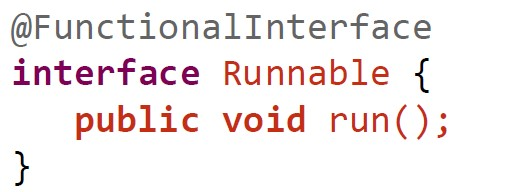
\includegraphics[width=0.7\linewidth]{pictures/runnable-interface.jpg}
        \end{minipage}
        \hfill
        \begin{minipage}{0.48\columnwidth}
            Kann auch als Lambda übergeben werden:\\
            \verb|Thread(Runnable task)|
        \end{minipage}
        Funktionsschnittstelle eines Threads, sie wird beim Starten des Threads durch die JVM gerufen.
        \vspace{-0.3cm}

    \subsubsection{Start und Ende $\qquad\qquad$ Thread ...}
        ... wird nach \verb|start()| ausgeführt (über \verb|run()| des \verb|Runnable|-Interfaces):\\
        \vspace{-0.3cm}
        \lstinputlisting{code/thread.java}
        \vspace{-0.1cm}
        ... endet beim Verlassen von \verb|run|, z.B. durch Ende der Methode, Return Statment oder unbeh. Exception
        \vspace{-0.3cm}

\subsection{Multi-Thread Beispiel}
    \vspace{-0.3cm}
    \lstinputlisting{code/Demo02MultiThread.java}
    \vspace{-0.2cm}

\subsection{Alternative Implementationen}
    \subsubsection{Explizit}
        \vspace{-0.3cm}
        \lstinputlisting{code/MyRunnable.java}
        \vspace{-0.2cm}

    \subsubsection{Sub-Klasse von Thread}
        \vspace{-0.3cm}
        \lstinputlisting{code/SimpleThread.java}
        \vspace{-0.2cm}

    \subsubsection{join()}
        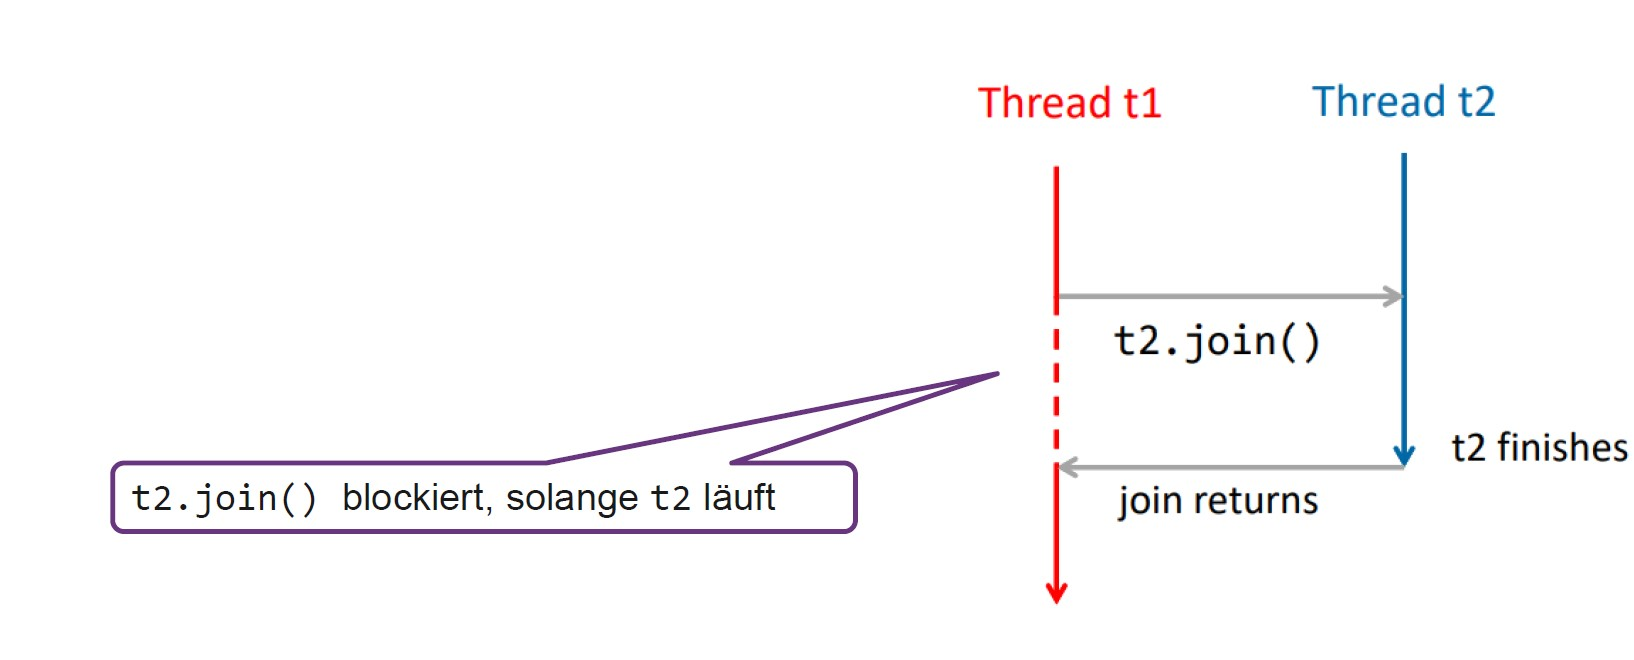
\includegraphics[width=0.6\linewidth]{pictures/thread-join.jpg}
        \vspace{-0.3cm}

\subsection{Thread-Methoden}
    \subsubsection{Thread Passivierung}
        \begin{tabular}{l}
            \textbf{Thread.sleep(milliseconds)} Laufender Thread put to sleep\\ \hline
            \textbf{Thread.yield()} Laufender Thread gibt Prozessor frei und\\
            $\qquad\qquad\qquad$ wird wieder ablaufbereit\\
        \end{tabular}
        \vspace{-0.3cm} 

    \subsubsection{InterruptedException}
        Mögliche Exception bei blockierenden Aufrufen, z.B. \verb|join(), sleep(), ...|

        Threads können von aussen unterbrochen werden: \verb|myThread.interrupt()| $\rightarrow$ bricht \verb|join(), sleep(), ...| ab
        \vspace{-0.3cm} 

    \subsubsection{Weitere Methoden}
        \vspace{-0.1cm} 
        \begin{tabular}{l}
            $\bullet$ \verb|static Thread currentThread()| liefert Instanz des Threads \\
            $\bullet$ \verb|long threadId()| liefert ID des Threads \\
            $\bullet$ \verb|void setDaemon(boolean on)| Thread als \textit{Daemon} markieren\\
        \end{tabular}
        \vspace{-0.3cm} 

\subsection{Synchronisation}
    \begin{tabular}{l}
        $\bullet$ Threads teilen sich Adressraum und Heap.\\
        $\bullet$ Wird auf dasselbe Objekt zugegriffen, muss abgesichert werden.\\
        $\bullet$ \verb|synchronized|: Modifier für Methoden, ähnlich wie ein Flag.\\
    \end{tabular}
    \vspace{-0.2cm} 
    \lstinputlisting{code/BankAccount.java}
    \vspace{-0.2cm}
    \tikz[baseline=(text.base)]\node[fill=orange, fill opacity=0.2, text opacity=1, rounded corners, inner sep=2pt, minimum height=5pt] (text) {Nur ein Thread kann eine der \verb|synchronized|-Methoden zur gleichen Zeit};
    \tikz[baseline=(text.base)]\node[fill=orange, fill opacity=0.2, text opacity=1, rounded corners, inner sep=2pt, minimum height=5pt] (text) {in derselben Instanz ausführen};
    \vspace{-0.2cm} 

}